\section{Discussion}
\label{sec:discussion}
  À partir des expériences de la section~\ref{sec:experiences},
  nous constatons la même échelle de difficulté quelque soit la méthode
  employée (cf. figure~\ref{fig:echelle}), ce qui montre que notre hypothèse de
  départ est valide. Il est toutefois important de noter qu'en observant les
  statistiques présentées dans le tableau~\ref{tab:statistiques_des_corpus},
  nous pouvons déduire la même échelle de difficulté à partir du rappel maximum.
  Cependant, le rappel maximum ne peut être obtenu en dehors d'un contexte
  expérimental. Dans cette section, nous nous fondons sur la nature des
  collections de données et sur les résultats de l'extraction non-supervisée de
  termes-clés pour déterminer quels sont les facteurs qui influent sur la
  difficulté de cette tâche.
  \begin{figure}
    \centering
    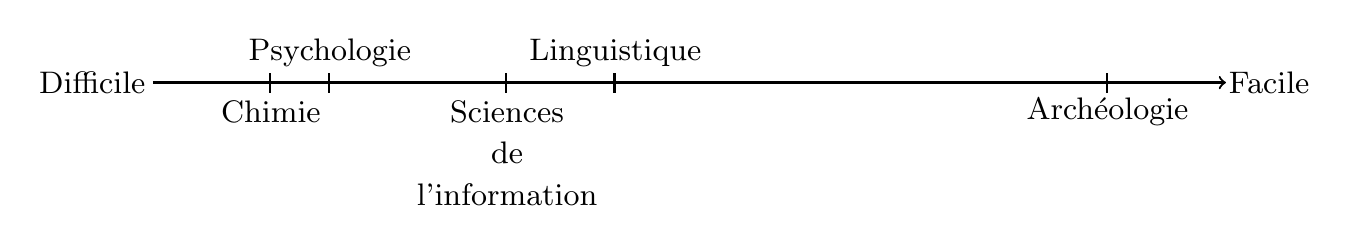
\begin{tikzpicture}[thin,
                        align=center,
                        scale=1.25,
                        every node/.style={text centered, transform shape}]
      \coordinate (start) at (4.5, 0);
      \coordinate (c) at (5.7, 0);
      \coordinate (p) at (6.3, 0);
      \coordinate (s) at (8.1, 0);
      \coordinate (l) at (9.2, 0);
      \coordinate (a) at (14.2, 0);
      \coordinate (end) at (15.4, 0);
      \node (chimie) at (5.7, -0.3) {\small Chimie};
      \node (psychologie) at (6.3, 0.3) {\small Psychologie};
      \node (sciences_de_l_information) at (8.1, -0.715) {\small Sciences\\\small de\\\small l'information};
      \node (linguistique) at (9.2, 0.3) {\small Linguistique};
      \node (archeologie) at (14.2, -0.3) {\small Archéologie};
      \draw[-|, thick] (start) node[xshift=-1.75em] (dificile) {\small Difficile} -- (c);
      \draw[-|, thick] (c) -- (p);
      \draw[-|, thick] (p) -- (s);
      \draw[-|, thick] (s) -- (l);
      \draw[-|, thick] (l) -- (a);
      \draw[->, thick] (a) -- (end) node[xshift=1.25em] (facile) {\small Facile};
    \end{tikzpicture}
    \caption{Échelle de difficulté disciplinaire, de la discipline la plus
             difficile à la discipline la plus facile à traiter par les méthodes
             d'extraction automatique de termes-clés.
             \label{fig:echelle}}
  \end{figure}

  Dans un premier temps, nous constatons que la pondération fondée sur la
  spécificité des mots améliore la stabilité (la robustesse) des méthodes
  d'extraction de termes-clés qui l'utilisent. Nous en déduisons que la nature
  linguistique des termes-clés utilisés dans une discipline est un facteur qui
  influe sur la difficulté de l'extraction des termes-clés. Ainsi, une forte
  tendance à l'usage de composés syntagmatiques constitués de mots centraux dans
  la discipline, tels que \og{}réaction\fg{} en Chimie (p.~ex. \og{}réaction
  topotactique\fg{} et \og{}réaction sonochimique\fg{}) ou encore le mot
  \og{}social\fg{}, qui est fréquemment utilisé en psychologie (p.~ex.
  \og{}interaction sociale\fg{} et \og{}environnement social\fg{}), augmente la
  difficulté de l'extraction des termes-clés.

  Dans un second temps, nous observons, sauf dans le cas de la psychologie,
  qu'il y a une correspondance entre l'ordre des disciplines selon la taille des
  résumés des notices et leur ordre dans l'échelle de difficulté. Ceci
  s'explique par la façon dont est organisé le discours dans les notices. Si
  nous prenons les notices d'archéologie, par exemple, celles-ci sont très
  détaillées. Il est par conséquent aisé d'établir des relations entre les
  concepts afin de déterminer quels sont ceux les plus importants, à la manière
  de TopicRank. À l'inverse, les notices de chimie, représentant principalement
  des comptes rendus d'expériences s'adressent à un lecteur expert pour lequel
  il est uniquement nécessaire de décrire le contexte expérimental. L'absence de
  détails dans les notices de certaines disciplines est donc un facteur qui
  influe sur la difficulté de l'extraction automatique de termes-clés,
  difficulté qui peut a priori être détectée à partir de la taille des notices.

